\documentclass[11pt]{ctexart}  
\usepackage[top=2cm, bottom=2cm, left=2cm, right=2cm]{geometry}  
\usepackage{algorithm}  
\usepackage{algorithmicx}  
\usepackage{algpseudocode}  
\usepackage{amsmath}  
\usepackage{graphicx}
  
\floatname{algorithm}{算法}  
\renewcommand{\algorithmicrequire}{\textbf{输入:}}  
\renewcommand{\algorithmicensure}{\textbf{输出:}}  
 

\begin{document}

\title{代数结构与组合数学·第二周作业} \author{刘方岳-2000013077} 
\maketitle

\section{15.9}
$x*y=x+y-xy=y+x+yx=y*x$,符合交换律,
$(x*y)*z=(x+y-xy)*z=x+y+z-xy-xz-yz+xyz=x*(y*z)$,符合结合律,
$x*x=x+x-x^2$不恒等于x,不符合幂等律.如$x=3$就不成立.

若存在单位元e,则$e*y=y$,则$e-ey=0$,故e=0.经验证,e为左、右单位元,故e=0为单位元.

若存在零元$\theta$,则$\theta * y=\theta$,故$y-\theta y =0$,从而$\theta=1$.经验证,$\theta$为左、右零元,故$\theta=1$为零元.

对于任意元素x,若$x*y=e$,则$x+y-xy=0$,故$y=\frac{x}{x-1}$,特别地,$x=1$是不可逆的.
$y*x=e$也成立,故对于可逆元素x($x\neq 1$),逆元为$\frac{x}{x-1}$.

\section{15.11}
不符合交换律,因为$<a,b>\circ <c,d>=<ac,ad+b>\neq <ac,cb+d> =  <c,d>\circ <a,b>$

$<a,b>\circ <c,d>\circ <e,f> = <ac,ad+b >\circ<e,f> = <ace,acf+ad+b >$.
$<a,b>\circ( <c,d>\circ <e,f>) = <a,b> \circ <ce,cf+d> =<ace,acf+ad+b>$.
故符合结合律.

设单位元为$<e_1,e_2>$,$<a,b>\circ <e_1,e_2> =<ae_1,ae_2+b> = <a,b>$,故$e_1=1,e_2=0$,
$<e_1,e_2>\circ <a,b> =<ae_1,be_1+e_2> =<a,b>$.
故单位元为$<1,0>$.

设零元为$<\theta_1,\theta_2>$,$<\theta_1,\theta_2>\circ <a,b> =<\theta_1,\theta_2>$.
故$\theta_1=0$.$<a,b> \circ <\theta_1,\theta_2>=<\theta_1,\theta_2>$.
造成无解.故无零元.

设$<a,b>$的逆元为$<c,d>$,由$<a,b>\circ <c,d>=<ac,ad+b>=<1,0>$,故c=$\frac{1}{a}$,$d=-\frac{b}{a}$.
$<ac,cb+d> =  <c,d>\circ <a,b>=<1,0>$成立.
故$<a,b>$当$a\neq 0$时可逆,逆元为$<\frac{1}{a},-\frac{b}{a}>$.

\section{15.14}
子代数:$<Z_6,\bigoplus >$,$<\{0\},\bigoplus>$,$<\{0,2,4\},\bigoplus >$,
$<\{0,3\},\bigoplus>$

平凡的子代数:$<Z_6,\bigoplus >$

真子代数:$<\{0,2,4\},\bigoplus >$,$<\{0,3\},\bigoplus>$,$<\{0\},\bigoplus>$


\section{15.16}


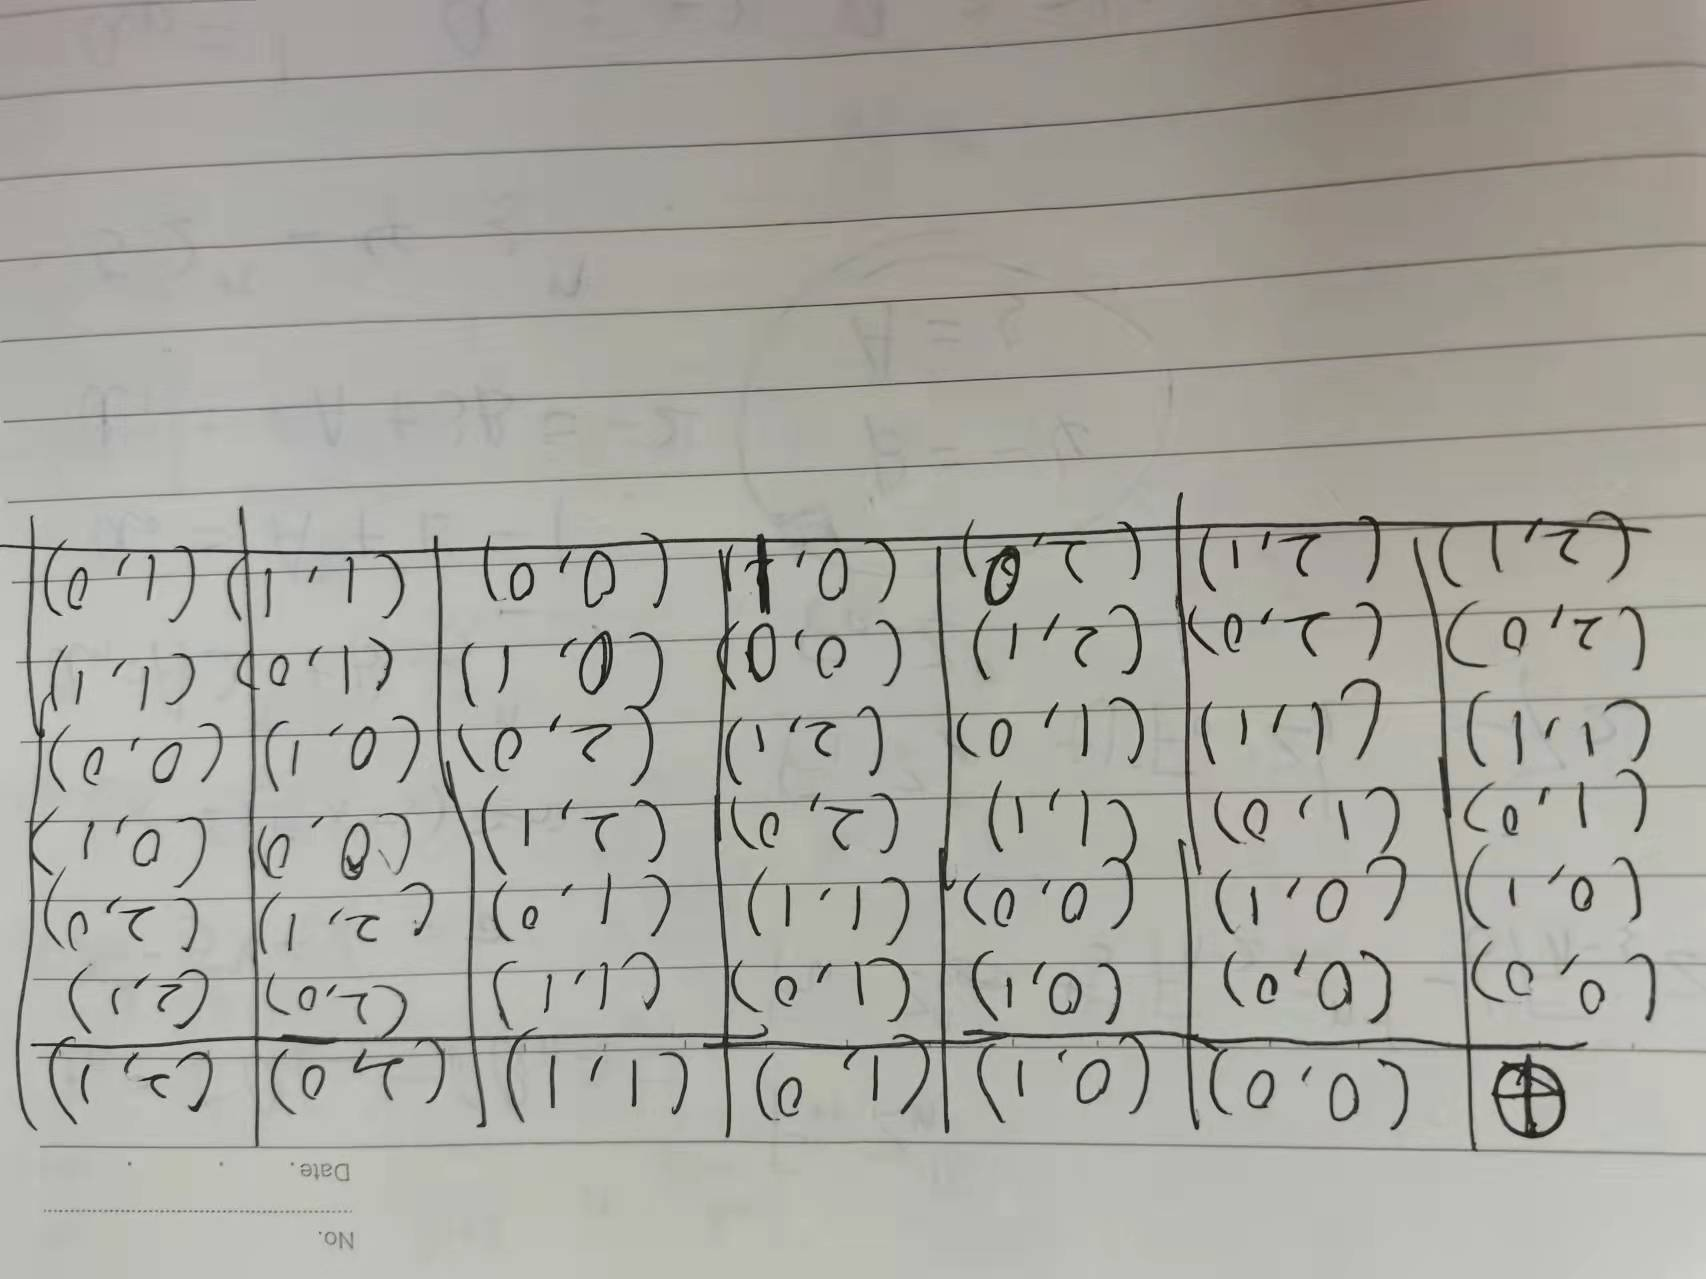
\includegraphics[angle=180,scale=0.2]{1.jpg}

单位元为$(0,0)$.
(0,0)逆元为(0,0),
(0,1)逆元为(0,1),
(1,0)逆元为(2,0),
(1,1)逆元为(2,1),
(2,0)逆元为(1,0),
(2,1)逆元为(1,1).


\section{15.18}

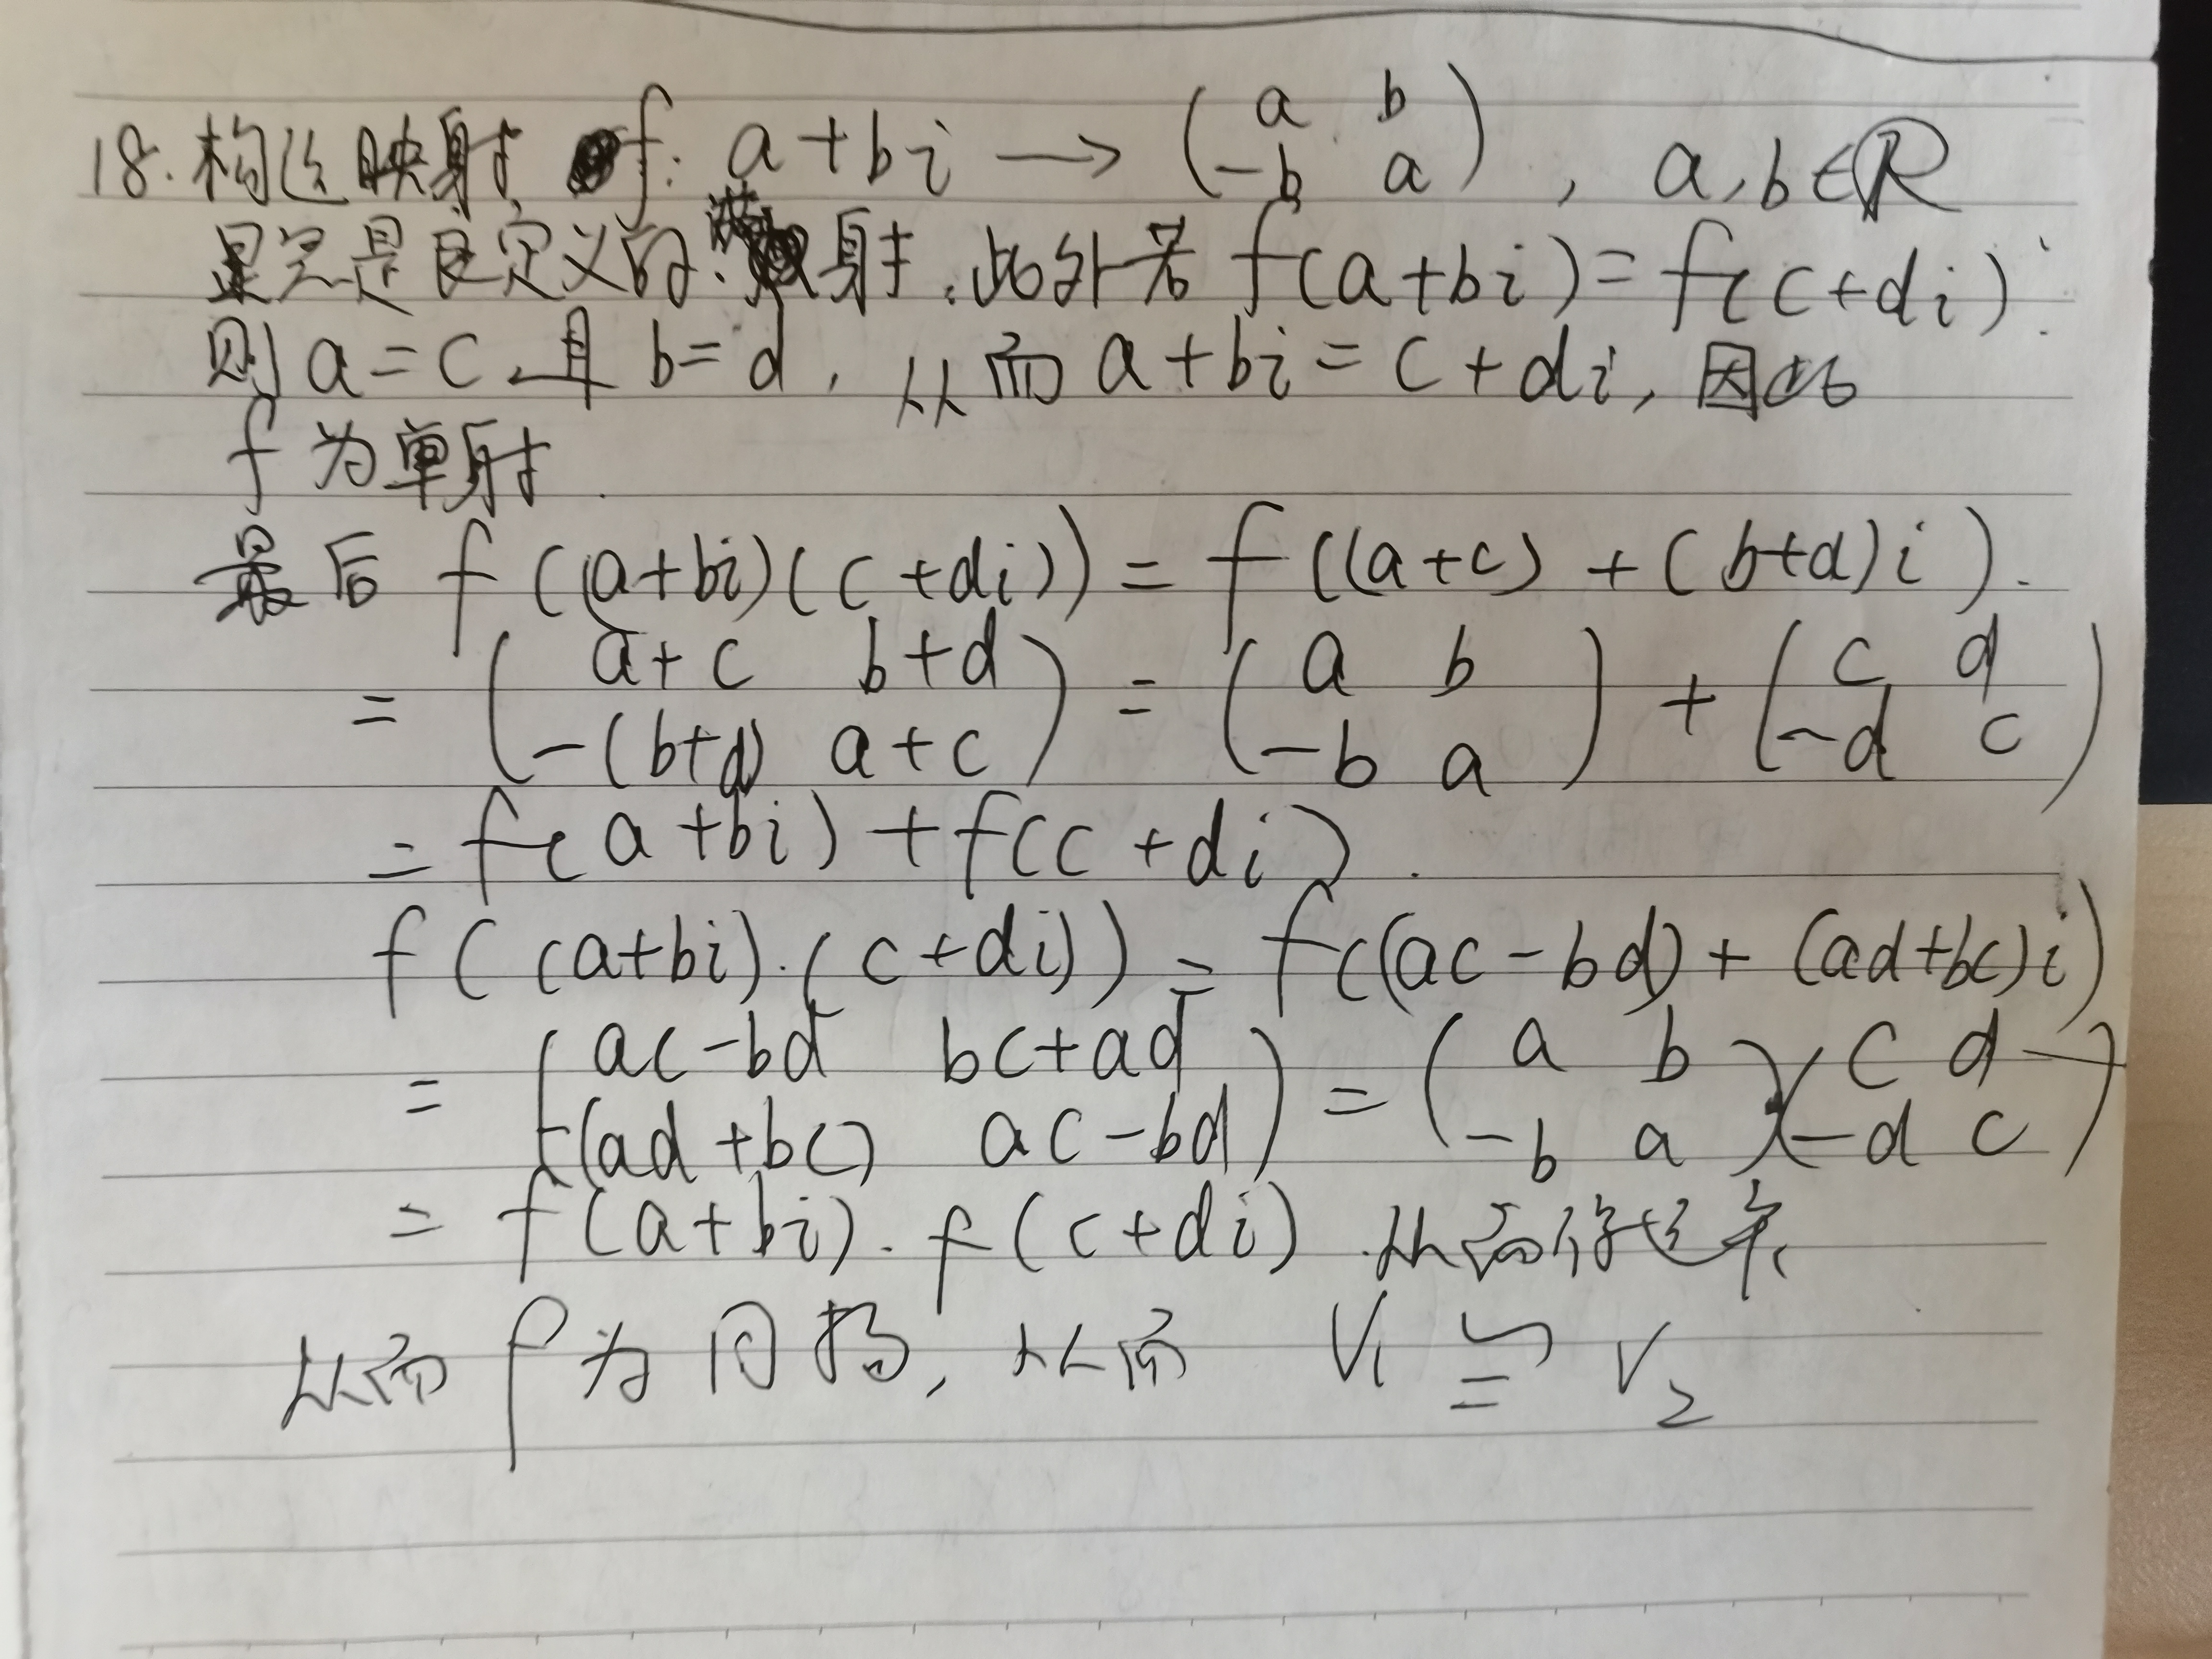
\includegraphics[scale=0.1]{2.jpg}



\section{15.24}

(1)不是同态.

(3)是同态. 同态像为$\{ 0 \}$.
其为良定义的映射.再证明其保运算,$\varphi(x\cdot y)=0=0\cdot 0=\varphi(x)\cdot \varphi(y)$.
零元运算也保持.故为同态.

\section{15.29}
\section{15.30}

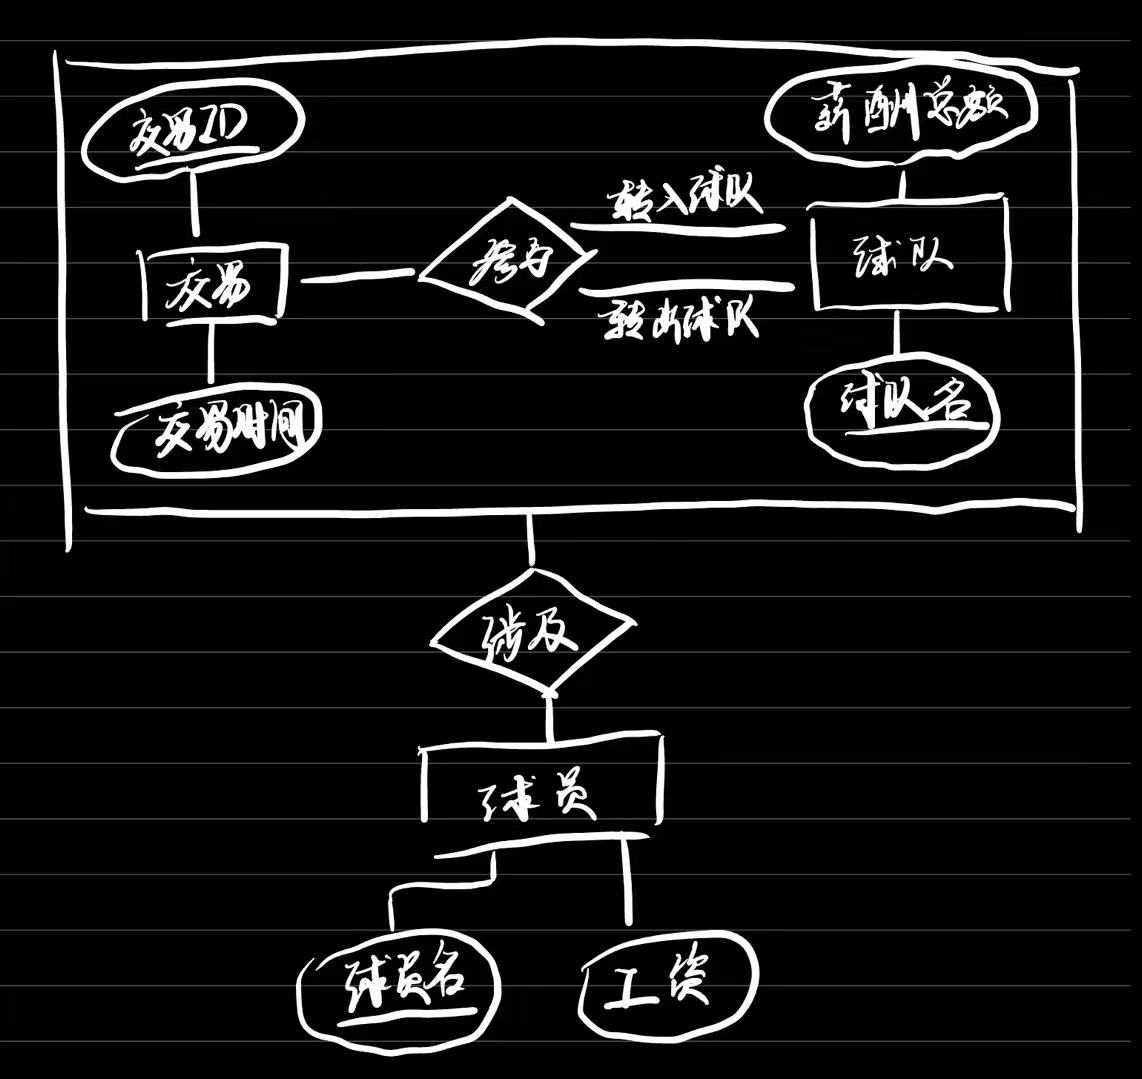
\includegraphics[scale=0.1]{3.jpg}




\end{document}  


	 